\chapter{Execution and Research}
\label{chap:execution}
\setstretch{1.5}
As a first step in the execution phase of the preliminary study, the programming environment needs to be set up. As the needed GPU-Voxels algorithm is only tested by the provider FZI Forschungszentrum Informatik on 64-bit Ubuntu 14.04 Linux Trusty and 16.04 Xenial systems, it was decided by the author to favor Ubuntu over Windows, but to use a newer Ubuntu distribution to work on a current system. Therefore, the newest version was chosen, which was at this point of time the version 18.04 Bionic Beaver LTS.
As programming IDE, Qt Creator was chosen, since this IDE was already used by the author during previous courses in robotics and informatics and is thus well known.
As a prerequisite for the GPU-Voxels algorithm, a CUDA compute capability greater than 2.0 is required. The compute capability of a GPU determines its general specifications and available features. This leads to the decision to use the authors private tower computer instead of the laptop used for the studies. The laptop couldn't be used because its onboard graphics card isn't supporting nVidia CUDA at all. Before week 12, start of the Bachelor Thesis, a Laptop with according performance shall be provided by the AHB to be used for this project.


\section{GPU-Voxels Algorithm\cite{voxels}}
\label{sec:voxels}
The GPU-Voxels algorithm was developed at the FZI Forschungszentrum Informatik in Karlsruhe, Germany. GPU-Voxels is a CUDA based library which allows a high resolution volumetric collision detection between animated 3D models and live point clouds from 3D sensors of all kind. Mainly developed for the use in robotics planning and monitoring tasks. The algorithm is able to voxelize 3D models and point clouds. By comparing voxel positions of the robot model and the point clouds, collisions can be accurately detected and visualized using third party visualizers \cite{GPU-Voxels}.

\subsubsection{Voxel}
A voxel is the three dimensional counterpart of the two dimensional pixel. As the pixel represents a certain area, depending on the resolution, in an XY-plane, a voxel represents a certain volume in an XYZ-space. Alongside its position a certain value can be assigned to a Voxel. This can be either binary, representing a simple free or occupied state, or multivalued, representing different data (e.g. color, density, heat or pressure).

\subsubsection{Point cloud}
A point cloud is a set of data points in a three-dimensional space, mostly representing the surface of an object or space. Based on how many points are used to create a point cloud, surfaces can be reconstructed very accurately. Typically, LIDARs or Stereo Cameras are used to gather Point Clouds.

\begin{figure}[h]
	\begin{center}
		\centering
		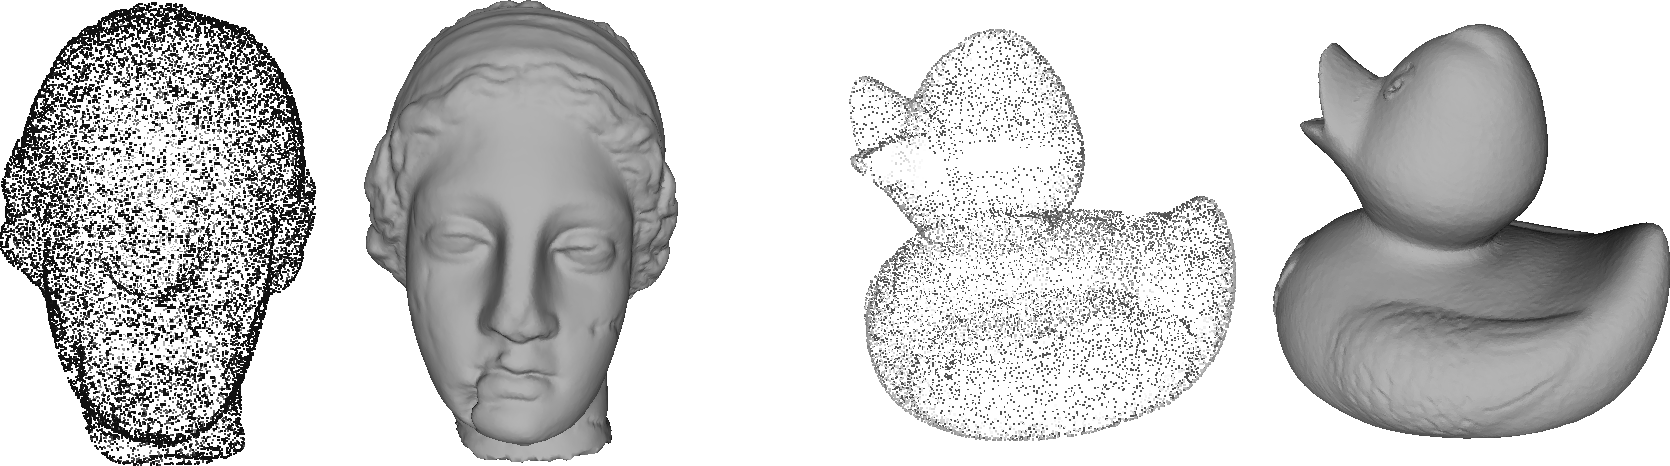
\includegraphics[width=1\linewidth]{images/point_cloud.png}
		\caption{Point Clouds and their reconstructed surfaces. \cite{fig:pc}}
		\label{fig:pointcloud}
	\end{center}
\end{figure}

\subsection{GPU-Voxels Prerequisites}
The GPU-Voxel Algorithm depends on several other Libraries which need to be installed in order to be able to compile GPU-Voxels. The following packages are necessary and must be available:

\setstretch{1.5}
\begin{itemize}
	\item \textbf{nVidia CUDA version 5.5 or higher} \newline CUDA enables many computing cores in a graphics processor to perform general-purpose mathematical calculations, which leads to dramatic speedups in computing performance.
	\item \textbf{Point Cloud Library (PCL)} \newline The Point Cloud Library is an open source library for 2D and 3D image and point cloud processing.
	\item \textbf{OpenNI} \newline OpenNI is an open source software development kit (SDK) used for applications for depth sensors such as Kinect and Asus Xtion.
	\item  \textbf{Boost} \newline Boost is a set of libraries for C++ that provides support for tasks and structures in linear algebra, pseudorandom number generation, multithreading and image processing. It contains over eighty individual libraries which are aimed at a wide range of C++ users.
	\item  \textbf{TinyXML} \newline TinyXML is an XML parser which converts data from an XML format in an in-memory form and creates a way for programs to use that data.
\end{itemize}
\setstretch{1.5}

In order to use the Visualizer further packages are necessary, but in a first installation they are not required and therefore not described in detail.
Installing the necessary packages, has proven difficult because some of them weren't compatible with each other. Sadly, no screenshots of the error message have been taken when occurred and are therefore now not available to be shown in this documentation. This is a finding, which the author now keeps in mind for the documentation of the Bachelor Thesis. 
While installing the nVidia CUDA Toolkit 10.0 the first time. Somehow the graphics driver was damaged, and a simple re-installation of the graphics driver didn't fix it. So, this led to a complete system re-install, with wiping the current Ubuntu partition and starting from Scratch.
In a second attempt all packages could be installed, and the only task left was compiling the GPU-Voxels algorithm. While compiling, cmake had problems finding packages, which was a time consuming but not unsolvable problem. During the step of fixing the package location in the cmake files of the GPU-Voxel Algorithm, several missing packages have been found. Most of them related to Robot operating System (ROS). ROS is an open-source operating System for robotics, which provides common functionality and services used in robotics. While GPU-Voxels state that their algorithm is independent from ROS, but it is supporting it, it was never possible to compile the code without ROS. Some of these packages were found as standalone packages, but couldn't be installed because of unmet dependencies, which lists several other packages and states that they are not going to be installed. This error could be avoided using the packages included in ROS. After installing the ROS Package, the graphics driver was damaged again. This lead again, to a clean start with a fresh Ubuntu installation, because a reinstallation of the graphics driver wouldn't fix the Problem.
In the third attempt the installation order of the packages was changed, and ROS was installed right after CUDA. Afterwards the other necessary packages were installed and compiling the GPU- Voxels Algorithm could start again. As before, some packages were still missing, but could not be installed because of unmet dependencies.
This whole process of trying to run the GPU-Voxels algorithm, was very time consuming and frustrating. A major mistake was, to lose focus on the whole project and how much time had already passed. In this process a lot of time was wasted without getting any results or achieving something. This phase made clear that the planning phase had failed, and the approach to the project was too straight forward directed to the main goal. Together with the missing documentation of the detailed errors and solutions, this Problem had a major influence on not being able to reach the set goals of this preliminary study.

\section{Looking for alternatives}
\label{chap:alternatives}
\setstretch{1.25}

After the struggles with the installation of the packages reached a critical point in terms of time that passed, a decision about the next steps had to be taken. Possible alternatives which allow a progress in this project needed to be found.

As a first step, the task which should be completed by the GPU-Voxel algorithm was divided in different functionalities. Functionality one is, that the workspace needs to be scanned and processed. Functionality two is, that the data from the workspace needs to be compared with the robot model and its trajectories, to predict collisions. Using the data from the collision prediction, a motion planning has to take place in order avoid collisions. To achieve these functionalities the search for packages began by looking into the packages the GPU-Voxel algorithm uses to solve these tasks. A few of them sounded promising, but the search was widened to other standalone libraries for each task to ensure a profound research with the best solution possible. The most promising ones are shortly explained in the following sections.

\subsection{Point Cloud Library \cite{Rusu_ICRA2011_PCL}}
The Point Cloud Library (PCL) supports the Microsoft Kinect cameras as well as the Asus Xtion Pro, which are available for this project. With this library it should be possible to create the necessary point clouds and process them into an octree data structure. The octree data structure was already mentioned in the documentation of the GPU-Voxels algorithm. PCL also provides efficient search routines.

\subsubsection{Octree data structure}

The octree is a tree data structure in which each internal node has exactly eight children. The root node describes a cubic bounding box which encapsulates all points from the point cloud. By
dividing this cube into eight smaller cubes each representing a certain part of the root cube. The node is always the center point of the cube it is representing. Processing a point cloud into an octree data structure already provides a form of voxelizing, the resolution can be chosen by defining how many layers the octree data structure should have.

\begin{figure}[!ht]
	\centering
	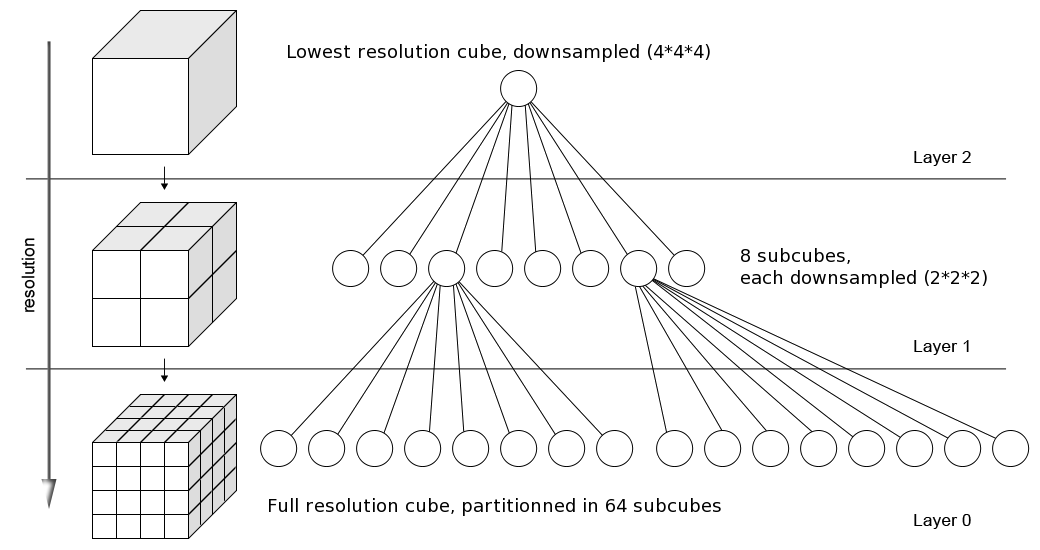
\includegraphics[width=0.6\linewidth]{images/Octree.png}
	\caption{Graphical Illustration of an octree data structure. \cite{fig:octree}}
	\label{fig:octree}
\end{figure}

\subsection{OctoMap \cite{hornung13auro}}
The Octomap library implements a 3D occupancy grid mapping approach, providing data structures and mapping algorithms in C++ suited for robotics. The implementation of the map is based on the previously explained octree data structure, which further allows map-based motion planning to take place.

\subsection{Open Motion Planning Library \cite{sucan2012the-open-motion-planning-library}}
The Open Motion Planning Library (OMPL) consists of many state-of-the-art sampling based motion planning algorithms, but does not contain anything related to collision checking or visualization. So, to use these motion planning algorithms, the collision detection needs to happen before the motion planning and the data needs to be provided accordingly. 

\section{Fanuc Roboguide and TCP/IP Socket messaging}
\label{chap:tcpip}
\setstretch{1.25}
\subsection{Roboguide}
Fanuc has its own simulation software for Fanuc robots called Roboguide. Roboguide provides the user with a complete and realistic simulation of the robot including teach pendant controls of robots. It can also be used to write the Karel programs, which will be later executed from the robot. With Roboguide, every aspect of the robot handling should be able to be simulated, including TCP/IP connections. Simulations are done in workcells, where a robot model can be included and an environment representing the actual robots environment can be created. So as a first step to learn how to use Roboguide, a new workcell was created, which was held very simple only including the robot model. Since it was said that the current physical environment of the robot was going to change in the near future, the work to model the current state was postponed till after the changes has been realized. After including the robot model into the workcell, a simple Karel program was written to move the Robot in a rectangular shape. This code has just been written, to learn some basic Karel functionality and syntax.

\subsection{TCP/IP}

As a first step, the existing work of a former student, Nino Sutter, has been analyzed. The work was provided via a gitlab repository, where access was granted as his work has showed similarities. The code provided should act as an example on how to enable a TCP/IP connection with the robot. The example has a Karel code which connects the robot with a system running a python program. Using the python program, tasks for the robot could be loaded remotely from the memory of the robot. A similar procedure is planned for this thesis. In order to provide the robot with coordinates for his destination point, a C++ program should calculate these and send them to the robot for movement commands. Technically it should be possible to adapt the Karel code from Nino Sutter to achieve the TCP/IP connection for this project on the Fanuc robot.
A first attempt using the example code to simulate a TCP/IP connection within Roboguide has not been successful. The reason for that may be found in missing settings inside the project work cell. But this was not further investigated due to timely limits of the preliminary study and the problems which occurred during GPU-Voxel algorithm setup.
Alternatively, the AHB has currently socket messaging, which is working on the robot for another project. This method of communication has not yet been reviewed, since the information came up in week 11 which is too close to the end of the preliminary studies due date. During the Bachelor Thesis this will be further analyzed to make sure to use the communication method that fits best \cite{motion}.


